\documentclass{article}

% ---------------------------------------------------------------------------
% NeurIPS style.  The official style file neurips_2025.sty sits next to this
% file.  "preprint" gives the non-anonymous layout without line numbers.
% To use another year's style file, change the name on the next line.
% ---------------------------------------------------------------------------
\usepackage[preprint]{neurips_2025}

% The style prints "Preprint." at the bottom of the first page.
% Say what this document is instead.
\makeatletter
\def\@noticestring{Final project report for AA228/CS238 (Decision Making under
  Uncertainty), Stanford University, Autumn 2026.}
\makeatother

\usepackage[utf8]{inputenc}
\usepackage[T1]{fontenc}
\usepackage{hyperref}
\usepackage{url}
\usepackage{booktabs}
\usepackage{amsmath}
\usepackage{amsfonts}
\usepackage{nicefrac}
\usepackage{microtype}
\usepackage{xcolor}
\usepackage{pgfplots}
\pgfplotsset{compat=1.17}

\hypersetup{colorlinks=true, linkcolor=black, citecolor=blue!45!black, urlcolor=blue!45!black}

% colours of the learning-curve figure
\definecolor{curveblue}{HTML}{2A78D6}
\definecolor{curveorange}{HTML}{EB6834}
\definecolor{plotgrid}{HTML}{E1E0D9}
\definecolor{plotaxis}{HTML}{898781}
\definecolor{plotink}{HTML}{52514E}

\title{Learning to Play Fish: A Per-Set Value Function\\
  for a Team Card Game with Hidden Information}

% ---------------------------------------------------------------------------
% E-mail addresses: replace the two placeholders on the next two lines.
% ---------------------------------------------------------------------------
\newcommand{\emailJonathan}{EMAIL-1@stanford.edu}
\newcommand{\emailMingchuan}{EMAIL-2@stanford.edu}

\author{%
  Jonathan Zhao \\
  Stanford University \\
  \texttt{\emailJonathan} \\
  \And
  Mingchuan Chen \\
  Stanford University \\
  \texttt{\emailMingchuan} \\
}

\begin{document}

\maketitle

\begin{abstract}
  Fish (also called Literature) is a six-player team card game in which players
  locate hidden cards by asking opponents for them and score by declaring
  exactly who holds every card of a set.  We treat it as a partially observable
  decision problem.  Every agent tracks what the public history proves with a
  constraint store, represents the remaining uncertainty by a weighted sample of
  complete deals, and chooses a move by one-step lookahead over its possible
  outcomes.  Within this framework we compare a hand-written evaluation of
  positions with one learned by TD($\lambda$) self-play.  A large network that
  reads every card separately and predicts the outcome of the game in a single
  number stayed at the level of a simple rule-based player.  A network with
  5,633 parameters that scores one set
  at a time from 21 summaries of the belief does: after 2,000 training games it
  beats the rule-based player by $3.40 \pm 0.24$ sets per game (out of nine) and
  the hand-written heuristic by $0.65 \pm 0.31$, each over 400 paired games.
  How the position is presented to the learner mattered far more than the
  amount of training.
\end{abstract}

\section{Introduction}

Fish, also known as Literature, is played by six players in two teams of three
with a 54-card deck divided into nine sets of six cards.  On a turn a player
asks one opponent for a specific card.  A team scores a set by \emph{declaring}
which of its members holds each of the six cards, and a wrong declaration gives
the set to the other team.  Every question and answer is public, so the game is
an exercise in inference: each ask reveals something about the asker's own
hand, a failed ask rules a card out of two hands, and a player must judge when
its team knows enough to declare before the opponents take the cards away.

Fish is a demanding test bed for decision making under uncertainty.  The
hidden state is large: at the start, one player's view is
consistent with $45!/(9!)^5 \approx 1.9 \times 10^{28}$ deals.  Observations
carry hard logical information as well as soft behavioural information, since
players tend to ask about sets in which they hold several cards.  Teammates
cannot communicate except through their public moves.  And a game lasts about
100 moves, while reward arrives only when a set is declared.

We build agents in three layers.  The first maintains everything that can be
\emph{proved} about the deal.  The second samples complete deals consistent
with those facts and weights them by how well they explain the asks seen so
far, which gives probabilities for where each card is.  The third evaluates
candidate moves by looking one step ahead: an ask succeeds or fails, a
declaration is right or wrong, and the value of each resulting position is
weighted by its probability.  All our agents share the first two layers.  They
differ in how a position is evaluated.\footnote{Code and training logs:
\url{https://github.com/mcc-cheng/fishy-RL}}

The paper makes three contributions: an environment for Fish with a sound
constraint store and a sampler of the deals consistent with it
(Sections~\ref{sec:game} and~\ref{sec:belief}); a value function factored into
one prediction per set, trained by TD($\lambda$) self-play after a warm start
on the games of a hand-written heuristic, which beats that heuristic
(Sections~\ref{sec:solver} and~\ref{sec:experiments}); and a negative result,
in that three variants of a single large network over per-card inputs stayed at
the level of a rule-based player with a similar budget
(Section~\ref{sec:experiments}).

\section{Related work}

Our training recipe is that of TD-Gammon \citep{tesauro1995}: a neural value
function over afterstates, trained on the $\lambda$-returns
\citep{sutton1988,suttonbarto2018} of self-play games and used with shallow
lookahead.  Later systems scaled self-play to deep networks and tree search
\citep{silver2018}; we use thousands of games on a single CPU.  Card games with
hidden information are often played by
determinization, which samples complete deals consistent with what is known and
solves each as if all cards were visible \citep{ginsberg2001,long2010}, despite
the problem of strategy fusion \citep{frank1998}, or by information-set Monte
Carlo tree search \citep{cowling2012}.  We also sample complete deals, but use
them as a particle belief in the sense of online POMDP planning
\citep{kaelbling1998,silver2010,kochenderfer2022}, to obtain outcome
probabilities and summary statistics.  Equilibrium-finding methods have reached
expert level in poker \citep{zinkevich2007,moravcik2017,brown2019}, an
adversarial game, and the Hanabi challenge \citep{bard2020} studies
cooperative play in which moves double as signals; Fish combines the two.  We
are not aware of published work on Fish itself.

\section{Fish as a decision problem}
\label{sec:game}

\paragraph{Rules.}
The deck is the 52 standard cards and two jokers, divided into nine sets of
six: the low cards (2--7) and the high cards (9--ace) of each suit, and the
four eights with the jokers.  Six players sit in a circle with
teammates alternating and receive nine cards each.  The player to move either
asks or declares.

An \emph{ask} names an opponent who holds at least one card, and a specific
card.  The asker must hold another card of the same set and must not hold the
card itself.  If the opponent has the card it changes hands and the asker moves
again; otherwise the turn passes to the opponent who was asked.

A \emph{declaration} names a set and, for each of its six cards, the teammate
who holds it.  If every card is where the declarer says, the declarer's team
scores the set; otherwise the other team does.  Either way the six cards leave
the game and the declarer keeps the turn.  A player without cards passes the
turn to the next teammate who has some.  The game ends when all nine sets have
been declared; a team's payoff is its sets won minus its sets lost, an odd
number from $-9$ to $9$.

Everything except the hands is public: every ask and its outcome, every
declaration and whether it was right, and the number of cards in each hand.
After a wrong declaration only the number of cards each player gives up is
revealed.

\paragraph{Formulation.}
The state consists of the owner of each card, the player to move, the sets
already declared and the score.  The only chance event is the initial deal, and
transitions are deterministic given the hidden hands.  Each player observes its
own hand and the public history.  With six decision makers and team payoffs
this is a partially observable stochastic game \citep{hansen2004}.  From the
point of view of one player, with the other five following fixed policies, it
is a POMDP \citep{kaelbling1998}, and this is the view we take: each agent
maintains a belief over deals and chooses moves to maximise its team's expected
final margin.  The action set is large because a set can be declared in
$3^6 = 729$ ways, but only a few moves are worth considering in any position
(Section~\ref{sec:solver}).

\section{Beliefs: what is certain and what is likely}
\label{sec:belief}

\paragraph{Constraint store.}
For every player $p$ the store holds the set of cards $p$ may hold, the hand
size, and a lower bound $m_{p,h}$ on the number of cards of each set $h$ in
$p$'s hand.  An ask by player $a$ for card $c$ of set $h$ shows that $a$ does
not hold $c$ and that $m_{a,h} \ge 1$.  If the ask fails, the player asked does
not hold $c$ either; if it succeeds, $c$ is now in $a$'s hand and the bounds
and hand sizes are adjusted.  A declaration removes its set.  After every
update, five inference rules are applied until nothing changes: (i)~a card with
a single possible holder is held by that player; (ii)~a player whose located
cards fill the hand holds nothing else; (iii)~a player who can hold only
$m_{p,h}$ cards of set $h$ holds all of them; (iv)~a player who can hold only
as many cards as the hand size holds all of them; and (v)~if the lower bounds
add up to the hand size, the player holds exactly $m_{p,h}$ cards of each set.
Every rule is sound, so the true deal always satisfies the store.  Each agent
keeps a private store, initialised with its own hand, and a public one without
it, which describes what everybody knows.

\paragraph{Sampled deals.}
The store leaves most cards unlocated, so an agent also samples $N$ complete
deals that satisfy it.  A sequential sampler assigns the unlocated cards one at
a time, most constrained first, choosing among the admissible holders in
proportion to their free capacity and recording the probability $q$ of the deal
it produces.  Resampling with weights $1/q$ corrects towards the uniform
distribution over consistent deals.  A Markov chain of pair swaps and
three-cycles, each accepted whenever the store remains satisfied, then removes
duplicates and residual bias; its proposals are symmetric, so the uniform
distribution is stationary.

\paragraph{Reading behaviour.}
Uniform weights ignore why players ask what they ask.  We model a player as
choosing the set to ask about with probability proportional to $k^{\alpha}$,
where $k$ is the number of cards of that set in the player's hand, and weight a
sampled deal $d$ by
\begin{equation}
  w(d) \;\propto\; \prod_{(a,h)} \max\{1,\, k_{a,h}(d)\}^{\alpha} ,
\end{equation}
where the product runs over the most recent asks (at most 60), each made by a
player $a$ in a set $h$, and $k_{a,h}(d)$ is the number of cards of $h$ that
$a$ held when asking if $d$ is the true deal.  This number can be reconstructed
because every later transfer is public.  We use $\alpha = 1$ throughout.  From
the weighted deals an agent reads off the probability that a given player holds
a given card, the most likely assignment of a set within its team, and the
summaries used in Section~\ref{sec:solver}.

\section{Baseline players}
\label{sec:baselines}

All players declare a set as soon as their store proves the declaration, and
guess when a declaration is forced because no ask is legal.  They differ in
everything else.

The \emph{rule-based} player asks for a card that it knows an opponent holds
whenever it may, choosing at random among such asks, and otherwise asks a
random legal question.

The \emph{heuristic} player uses the weighted deals of
Section~\ref{sec:belief}.  It scores an ask of opponent $j$ for a card that $j$
holds with probability $p$ as
\begin{equation}
  p\,g \;-\; (1-p)\,\tau_j , \qquad g = \tfrac{1}{3} ,
\end{equation}
where $g$ is the worth of one card when a set is scored from $-1$ (the
opponents hold all six cards) to $+1$.  The threat
$\tau_j = g \max_h e_h\,\pi_{j,h}$ estimates what $j$ can take back with the
turn: $\pi_{j,h}$ is the probability that $j$ holds a card of set $h$ and may
therefore ask about it, and $e_h$ is the largest probability with which public
information places a card of $h$ in the hand of one particular member of the
asker's team.  Declaring set $h$ with its most likely assignment, of
probability $q$, scores $(2q-1) - u_h$, where $u_h \in [-1,1]$ is the current
worth of the set, computed from the expected number of its cards held by the
team.  The heuristic plays the highest-scoring move.  It looks one step ahead
with fixed formulas, and nothing in it is learned.

\section{A learned evaluation}
\label{sec:solver}

The learned player, which we call the \emph{solver}, keeps the belief layers
and the one-step lookahead but replaces the heuristic's formulas with a value
function trained from games.

\paragraph{Describing a position one set at a time.}
We do not present the whole position to one network.  Each undeclared set $h$
is described by a vector $\phi_h(b) \in [0,1]^{21}$ computed from the player's
belief $b$, that is, from its two stores and its weighted deals
(Table~\ref{tab:features}).  Thirteen entries describe the set and eight
describe the position as a whole.  All are expressed relative to the player
(``my team'', ``the opponents''), so one function serves all six seats, and
none refers to a particular card or suit, so the same function serves all nine
sets.

\begin{table}[t]
  \caption{The 21 inputs that describe one set $h$ from one player's point of
    view, all in $[0,1]$ (card counts are divided by six).  Probabilities and
    expectations are over the weighted deals of Section~\ref{sec:belief}.}
  \label{tab:features}
  \centering
  \small
  \begin{tabular}{@{}rp{0.87\linewidth}@{}}
    \toprule
    \multicolumn{2}{@{}l}{\emph{About the set}} \\
    1 & Cards of $h$ in the player's own hand \\
    2 & Expected number of cards of $h$ held by the player's team \\
    3--4 & Probability that the team holds all six cards; that the opponents do \\
    5--6 & Cards of $h$ that the player can place with certainty in its own team; in the other team \\
    7--8 & The same two counts using public knowledge only \\
    9--10 & Public lower bound on the cards of $h$ held by the team; by the opponents \\
    11--12 & Probability that the player to move holds a card of $h$; expected number of such cards \\
    13 & If the player is to move: the highest success probability among its asks for cards of $h$ \\
    \midrule
    \multicolumn{2}{@{}l}{\emph{About the whole position (repeated for every set)}} \\
    14--16 & Who is to move: the player, a teammate, or an opponent \\
    17 & Fraction of the nine sets still undeclared \\
    18--19 & Hand size of the player; of the player to move (divided by 18) \\
    20 & Share of the cards still in play that the team holds \\
    21 & If the player is to move: the highest success probability among all its asks \\
    \bottomrule
  \end{tabular}
\end{table}

\paragraph{Value function and choice of move.}
A network $v_\theta : [0,1]^{21} \to (-1,1)$ predicts how one set will end for
the player's team: $+1$ if the team wins it and $-1$ if it loses it.  The
network has two hidden layers of 64 rectified linear units and a $\tanh$
output, 5,633 parameters in total.  The value of a position is the score so far
plus the predictions for the sets still in play,
\begin{equation}
  V_\theta(b) \;=\; \frac{1}{9}\Bigl(\Delta(b) + \sum_{h \in \mathcal{L}(b)} v_\theta\bigl(\phi_h(b)\bigr)\Bigr) ,
  \label{eq:value}
\end{equation}
where $\Delta(b)$ is the current score difference and $\mathcal{L}(b)$ the set
of undeclared sets.

To move, the solver scores each candidate $a$ by its expected value one step
ahead,
\begin{equation}
  Q(b,a) \;=\; p_a\,V_\theta(b_a^{+}) + (1-p_a)\,V_\theta(b_a^{-}) .
  \label{eq:lookahead}
\end{equation}
For an ask, $p_a$ is the probability that the opponent holds the card,
$b_a^{+}$ is the belief after a success and $b_a^{-}$ the belief after a
failure, in which the turn has passed to that opponent.  Each is obtained by
applying the hypothetical observation to the stores and keeping the sampled
deals in which that outcome occurs.  For a declaration, $p_a$ is the
probability of the most likely assignment, multiplied by
$n_{\mathrm{eff}}/(n_{\mathrm{eff}}+1)$, where
$n_{\mathrm{eff}} = 1/\sum_n w_n^2$ is the effective sample size, so that an
unproven declaration is never treated as certain.  The candidates are the ten
asks most likely to succeed and, for every set that the team may hold
completely, its most likely declaration.  A declaration that the store proves
correct is played at once.

\paragraph{Training.}
The network is trained with TD($\lambda$) on afterstates.  After each move we
record the resulting position from the mover's point of view, that is,
$\phi_h$ for every undeclared set.  When a set is declared, the team that
scores it receives a reward of $+1$ for that set and the other team $-1$.  Let
$b_1, \dots, b_K$ be the recorded positions of a game.  Writing everything from
one team's side, the target for set $h$ at position $k$ is the
$\lambda$-return
\begin{equation}
  G^h_k \;=\; R^h_k + (1-\lambda)\,v_\theta\bigl(\phi_h(b_{k+1})\bigr) + \lambda\,G^h_{k+1} ,
  \label{eq:target}
\end{equation}
where $R^h_k$ is the reward for set $h$ received between positions $k$ and
$k+1$, and both the prediction and the return are zero beyond the last
position.  Predictions made from the other team's seats enter with the opposite
sign.  Targets are computed when the game ends and are stored with the
positions in a replay memory of 40,000 positions \citep{lin1992}.  After each
game the network takes 16 Adam steps \citep{kingma2015} with learning rate
$10^{-3}$ and batches of 256 positions on the squared error, averaged over
undeclared sets.  Training games are stopped after 300 moves, and sets still
undeclared at that point yield no reward.

Training games are produced in two phases.  In the first 200 games, the
\emph{warm start}, all six seats are played by the heuristic and $\lambda = 1$,
so the network learns to predict how sets end under the heuristic's play.  In
the remaining 1,800 games the network chooses the moves.  In 70\% of these
games it plays all six seats.  In the other 30\% its team plays a team of
heuristic players, and only the network's own positions are recorded.  Here
$\lambda = 0.9$, and with probability $\varepsilon$ a random candidate ask is
played instead of the best move, with $\varepsilon$ decreasing linearly from
$0.10$ to $0.02$.  The solver samples $N = 48$ deals per decision and the
heuristic 100.  The implementation uses Python with PyTorch
\citep{paszke2019}; generating and learning from the 2,000 games took 53
minutes on a laptop CPU.

\section{Experiments}
\label{sec:experiments}

\paragraph{Protocol.}
We compare two players by seating one at the even seats and the other at the
odd seats.  Because the deal strongly affects the result, every deal is played
twice with the teams exchanged and the two results are averaged.  We report the
mean set margin per game (sets won minus sets lost, out of nine) with a 95\%
confidence interval over deals (normal approximation), and the fraction of
games won.  An evaluation uses 200 deals, that is, 400 games, unless stated
otherwise.  The solver plays greedily with $N = 48$, the heuristic uses
$N = 150$, and games are stopped after 3,000 moves.

\begin{table}[t]
  \caption{The solver after 2,000 training games against each baseline, over
    400 games on 200 deals.  Margins are in sets per game, with 95\% confidence
    intervals over deals.}
  \label{tab:main}
  \centering
  \begin{tabular}{lccc}
    \toprule
    Opponent & Set margin & Games won & Median game length \\
    \midrule
    Rule-based & $+3.40 \pm 0.24$ & 366 of 400 (92\%) & 107 moves \\
    Heuristic  & $+0.65 \pm 0.31$ & 231 of 400 (58\%) & 96 moves \\
    \bottomrule
  \end{tabular}
\end{table}

\paragraph{Main result.}
Table~\ref{tab:main} shows the solver after 2,000 training games.  It wins 92\%
of its games against the rule-based player with an average margin of 3.40 sets
(an average score of about 6.2 to 2.8).  Against the heuristic it wins 58\%
with a margin of $0.65 \pm 0.31$ sets (about 4.8 to 4.2).  The interval
excludes zero, but the edge is small next to the spread of a single game, whose
margin has a standard deviation of about three sets.  The solver achieves it
with a third as many sampled deals per decision as the heuristic.  One game
against the heuristic had not ended after 3,000 moves and is counted with the
sets scored up to then.

\begin{figure}[t]
  \centering
  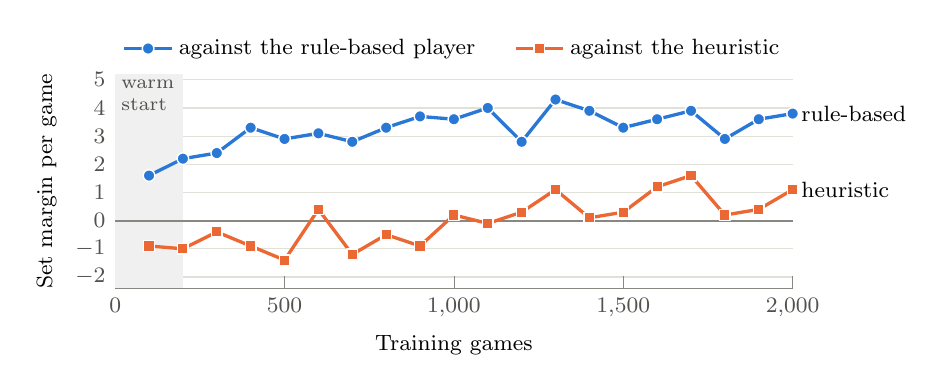
\begin{tikzpicture}
    \begin{axis}[
        width=0.84\linewidth, height=4.3cm,
        xmin=0, xmax=2000, ymin=-2.4, ymax=5.2,
        xtick={0,500,1000,1500,2000},
        xticklabels={0,500,{1,000},{1,500},{2,000}},
        ytick={-2,-1,0,1,2,3,4,5},
        scaled x ticks=false,
        xlabel={Training games},
        ylabel={Set margin per game},
        axis x line*=bottom, axis y line*=left,
        axis line style={draw=plotaxis},
        tick style={draw=plotaxis},
        tick label style={font=\footnotesize, text=plotink},
        label style={font=\footnotesize},
        ymajorgrids, major grid style={draw=plotgrid, line width=0.4pt},
        clip=false,
        legend columns=2,
        legend style={font=\footnotesize, draw=none, fill=none,
          at={(0.5,1.02)}, anchor=south, legend cell align=left,
          /tikz/every even column/.append style={column sep=1.2em}},
      ]
      % warm start: the heuristic plays every seat
      \fill[black!6] (axis cs:0,-2.4) rectangle (axis cs:200,5.2);
      \node[anchor=north west, font=\scriptsize, text=plotink, align=left, inner sep=2pt]
        at (axis cs:0,5.2) {warm\\start};
      % level with the opponent
      \draw[draw=plotaxis, line width=0.8pt] (axis cs:0,0) -- (axis cs:2000,0);
      \addplot[color=curveblue, line width=1.2pt, line join=round, mark=*, mark size=2.1pt,
          mark options={draw=white, fill=curveblue, line width=0.5pt}]
        coordinates {(100,1.6) (200,2.2) (300,2.4) (400,3.3) (500,2.9) (600,3.1) (700,2.8)
          (800,3.3) (900,3.7) (1000,3.6) (1100,4.0) (1200,2.8) (1300,4.3) (1400,3.9)
          (1500,3.3) (1600,3.6) (1700,3.9) (1800,2.9) (1900,3.6) (2000,3.8)};
      \addlegendentry{against the rule-based player}
      \addplot[color=curveorange, line width=1.2pt, line join=round, mark=square*, mark size=1.9pt,
          mark options={draw=white, fill=curveorange, line width=0.5pt}]
        coordinates {(100,-0.9) (200,-1.0) (300,-0.4) (400,-0.9) (500,-1.4) (600,0.4) (700,-1.2)
          (800,-0.5) (900,-0.9) (1000,0.2) (1100,-0.1) (1200,0.3) (1300,1.1) (1400,0.1)
          (1500,0.3) (1600,1.2) (1700,1.6) (1800,0.2) (1900,0.4) (2000,1.1)};
      \addlegendentry{against the heuristic}
      \node[anchor=west, font=\footnotesize, inner sep=3pt] at (axis cs:2000,3.8) {rule-based};
      \node[anchor=west, font=\footnotesize, inner sep=3pt] at (axis cs:2000,1.1) {heuristic};
    \end{axis}
  \end{tikzpicture}
  \caption{Learning curve of the main run.  Every 100 training games the
    current network plays 20 test games against each baseline on ten fixed
    deals, so the level of each curve is uncertain by more than one set.  The
    first 200 games (shaded) are played by the heuristic.}
  \label{fig:curve}
\end{figure}

\paragraph{Learning curve.}
During training the current network is tested every 100 games on ten fixed
deals, each played from both sides (Figure~\ref{fig:curve}).  After the warm start alone, when it has
only watched the heuristic play, the network already beats the rule-based
player by about two sets but loses to the heuristic by one.  Self-play raises
both curves.  The solver draws level with the heuristic after about 1,000 games,
and both curves are flat within their noise from about 1,300 games on.

\begin{table}[t]
  \caption{Earlier designs and the per-set design.  A and B: 100 games per
    opponent.  C was stopped early and never evaluated formally; its entries
    average thirteen ten-game tests made during training.}
  \label{tab:designs}
  \centering
  \small
  \begin{tabular}{@{}lp{0.37\linewidth}rrcc@{}}
    \toprule
    & Input and training signal & Inputs & Parameters & vs.\ rule-based & vs.\ heuristic \\
    \midrule
    A & Constraint store; final result only & 725 & 251,905 & $-0.10 \pm 0.61$ & $-3.52 \pm 0.49$ \\
    B & As A, plus a reward per declaration & 725 & 251,905 & $+0.54 \pm 0.53$ & $-2.94 \pm 0.60$ \\
    C & As B, plus card probabilities, warm start and heuristic opponents & 1,049 & 334,849 & $-0.2$ & $-3.8$ \\
    \midrule
    & Per-set design (Section~\ref{sec:solver}) & $9 \times 21$ & 5,633 & $+3.40 \pm 0.24$ & $+0.65 \pm 0.31$ \\
    \bottomrule
  \end{tabular}
\end{table}

\paragraph{Earlier designs.}
Before arriving at the per-set design we trained three variants of a more
conventional one: a single network with two hidden layers of 256 units that
reads the whole position and outputs the predicted margin.  Variant A reads the
constraint store itself (for every seat and card, whether the card is certainly
held and whether it may be held, plus hand sizes, lower bounds, declared sets,
score and turn; 725 numbers) and learns from the final result of 2,000
self-play games.  Variant B instead receives a reward at each declaration.
Variant C adds the sampled probability of every card in every hand, the warm
start and the heuristic opponents; we stopped it after 650 games.

None of the three beat the rule-based player by a meaningful margin, and all
lost to the heuristic by about three sets or more (Table~\ref{tab:designs}).
The cause was not a failure to fit.  During the warm start of variant C, where
the targets are actual outcomes, its training error was between 0.002 and
0.004 in units in which the final margin has a variance of about 0.1.  A
network with $3 \times 10^5$ parameters can memorise the outcomes of a few
hundred games, and what it memorises says little about which of two similar
moves is better.

\paragraph{Longer training.}
Continuing the main run to 3,000 and then 5,000 games ($\varepsilon = 0.02$,
learning rate $3 \times 10^{-4}$) did not improve the solver.  On the same 200
deals the later networks score $+3.42 \pm 0.25$ and $+3.54 \pm 0.27$ against
the rule-based player and $+0.40 \pm 0.31$ and $+0.39 \pm 0.27$ against the
heuristic, and the paired differences from the 2,000-game network are within
noise ($-0.27 \pm 0.40$ for the 5,000-game network against the heuristic).  We
therefore keep the planned 2,000-game network as the main result; together the
three evaluations put its edge over the heuristic at $0.48 \pm 0.18$ sets.

\section{Discussion}

\paragraph{Why the per-set design learns.}
Several things changed between variant C and the per-set design, so we cannot
attribute the improvement to one of them, but three properties seem important.
First, the weights are shared: every game yields nine set outcomes, each seen
from about a hundred positions, and all of them train the same small function,
whereas a network over raw cards must discover separately that the game treats
all suits, all cards of a set and all seats alike.  Second, the targets are
less noisy: the final margin has a standard deviation of about three sets, most
of it due to the deal, whereas the fate of one set depends mainly on the
quantities in Table~\ref{tab:features}.  Third, 5,633
parameters cannot memorise 40,000 positions.  As for the gain over the
heuristic, both players rank asks with the same probabilities, but the
heuristic gives every card the same worth and prices the loss of the turn with
a fixed formula, whereas the network lets both depend on the position.  We have
not analysed which situations account for the gain.

\paragraph{Limitations.}
The main result comes from a single training run.  All opponents are our own
baselines, and the heuristic is both training partner and yardstick, so part of
the edge may be specific to it.  We ran no ablations that separate the
contributions of the warm start, of self-play and of the heuristic opponents.
The solver looks only one move ahead, does not model what its teammates know,
and assumes one simple behaviour model for everybody's asks.

\section{Conclusion}

We built agents that play Fish by exact logical tracking, a sampled belief and
one-step lookahead, and showed that within this pipeline a small learned
evaluation outperforms a hand-written one: after 2,000 training games the
solver wins 58\% of its games against the heuristic ($0.65 \pm 0.31$ sets per
game) and 92\% against a rule-based player.  The decisive step was neither more
data nor a larger network but a change of representation, predicting the fate
of each set from a few summaries of the belief with weights shared across sets
and seats.  Longer training did not help, so further gains are more likely to
come from what the evaluation sees and from how far the search looks ahead.

% TODO (authors): if the course asks for it, add a short statement of who did what.
% \section*{Contributions}

{\small
\setlength{\bibsep}{4pt plus 1pt}
\bibliographystyle{plainnat}
\bibliography{references}
}

\end{document}
